\newpage
\section{Smart meter types}

Main question: What types of outputs are there for smart meters to transfer data.

\subsection{Hypothesis}
Different smart meters use different types of output types. These output types are
\begin{itemize}
    \item Ethernet
    \item USB
    \item RJ11
    \item RS485
\end{itemize}
These outputs need to be able to connect to the router which will be modular.

\subsection{Sub questions}
\begin{enumerate}
    \item What is a smart meter?
    \item What are the uses of a smart meter?
    \item What are the different types of smart meters?
    \item What are the different outputs for the smart meters?
    \item What are the costs for the outputs?
\end{enumerate}

\subsection{Methodology}
\subquestion{1}{What is a smart meter?}{2}
This will be researched by reading articles that talk about smart meters.

\subquestion{2}{What are the uses of a smart meter?}{2}
The uses will be researched by reading scientific articles.

\subquestion{3}{What are the different types of smart meters?}{2}
Research the biggest manufacturers in order to see what kind of smart meters are made.

\subquestion{4}{What are the different outputs for the smart meters?}{2}
same as sub-question 3.

\subquestion{5}{What are the costs for the outputs?}{2}
Compare the different types of outputs

\subsection{What is a smart meter?}
\textit{"A smart meter is one of the most important devices used in a smart grid."}\cite{SmartMeterInfo}. So to understand the smart meter the smart grid must first be understood. \textit{The Smart Grid, regarded as the next generation power grid, uses two-way flows of electricity and information to create a widely distributed automated energy delivery network}\cite{smartGrid}. It is also important to know that the smart grid has to be integrated to the current grid\cite{SmartHomeSmartGrid}. The difference between the grids is seen in \autoref{tab:smart_grid} The smart grid term is widely acceptable for the grid including wire line and wireless communication structures. The smart meter helps with the communication and the measurements in the smart grid which makes it an essential part.

\begin{table}[H]
    \centering
    \begin{tabular}{|c|c|}\hline
        \textbf{Existing grid} & \textbf{Smart grid}\\\hline
        Electromechanical& digital \\\hline
        One-way communication & Two-way communication \\\hline
        Centralized generation & Distributed generation \\\hline
        Few sensors & Sensors throughout\\\hline
        Manual monitoring & Self monitoring \\\hline
        Manual restoration& Self-Healing \\\hline
        Failures and blackouts & Adaptive and islanding \\\hline
        Limited control & Pervasive control\\\hline
        Few customer choices & Many customer choices \\\hline
    \end{tabular}
    \caption{Differences between Existing and smart grid\cite{SmartMeterInfo}}
    \label{tab:smart_grid}
\end{table}

\subsection{Uses smart meter}
The main thing a smart meter is used for is energy consumption measurement and control. One of the uses can be for internet of things\cite{SmartMeterIOT} this entails that smart meters can also connect with each other and exchange information. This of course is one option. As it is show the smart meter qua data is only using energy data. There are many ways to use smart meter for monitoring for electricity theft\cite{SmartMeterTheft} for example. It can also monitor the gas and heat used in a home.
\begin{figure}[H]
    \centering
    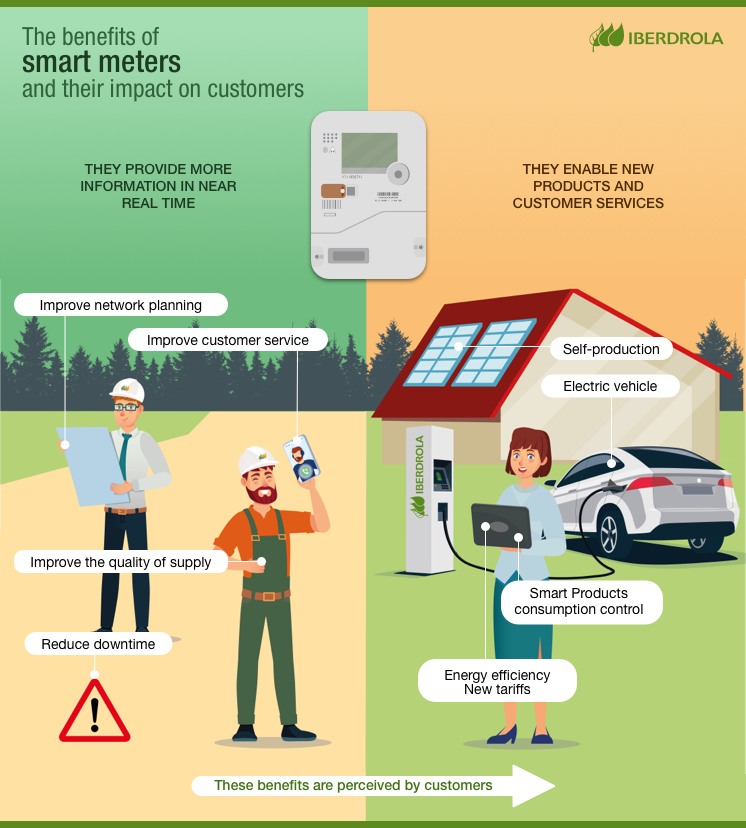
\includegraphics[width=10cm]{Images/Research/Infographic_Smart_Meters_EN.jpg}
    \caption{Uses smart meter\cite{FigureSM}}
    \label{fig:uses_smart_meter}
\end{figure}

\subsection{Types of smart meters}
There are many different types of smart meters. The specific meters are smart current meter, smart gas meter, smart water meter and smart heat meter\cite{DiffSMeters}. There are also combo's of this of course. Now there will be looked at the biggest companies that sell smart meters.

\begin{table}[H]
    \hspace{-2.0cm}
    \begin{tabular}{|p{1.5cm}|p{3.8cm}|p{2.7cm}|p{6cm}|p{2.9cm}|}\hline
        \textbf{Number} & \textbf{Electric meters}\cite{TOP10ELECMET} & \textbf{Gas meters}\cite{TOP10GASMET} & \textbf{Heat meters}\cite{TOP10HEATMET}& \textbf{Water meters}\cite{TOP10WATERMET}\\\hline
        1 & Sensus & Elster & Siemens AG & Anglian water\\\hline
        2 & Landis \+ Gyr & General electric & Danfoss& Itron\\\hline
        3 & Itron Inc. & Itron & Diehl Group& Laison\\\hline
        4 & Sojitz co., Ltd & Landis \+ Gyr & Wassion Group Co. Ltd.&Camwater \\\hline
        5 & Exelon & ABB &  Landis \+ Gyr&WEGoT\\\hline
        6 & NES & Aclara & Itron Inc.&Ameresco\\\hline
        7 & Allete, Inc. & Badget meter & IstaInternational GmbH&Business Stream\\\hline
        8 & Honeywell International& Actatis & Elster Group&Thames Water\\\hline
        9 & Scottish power& Diehl metering& Zenner International GmbH \& Company&United Utilities\\\hline
        10 & Siemens & Krohne & Kamstrup&Global Omnium\\\hline
    \end{tabular}
    \caption{Meter companies}
    \label{tab:Meter_companies}
\end{table}

\subsection{Outputs}
By searching what kind of communication is used by smart meters more connections can be found. It is shown in the list below.

\begin{itemize}
    \item Ethernet\cite{ConnectionsSmartMeter}\cite{ConnectionsSmartMeter2}
    \item Power Line Communication\cite{ConnectionsSmartMeter}\cite{ConnectionsSmartMeter2}
    \item Meter bus\cite{ConnectionsSmartMeter}
    \item Digital Subscriber Line \cite{ConnectionsSmartMeter2}
\end{itemize}